\documentclass{article}
\usepackage[utf8]{inputenc}
\usepackage[czech]{babel}
%\usepackage[T1]{fontenc}
\usepackage[autostyle]{csquotes}

\usepackage{graphicx}
\usepackage{amsmath}
\usepackage{amssymb}
\usepackage{geometry}
\usepackage{graphicx}
\usepackage{epstopdf}
\usepackage{caption}
\usepackage{subcaption}
\usepackage{float}
\usepackage{xcolor}
\usepackage{gensymb}
\usepackage{hyperref}
\usepackage{physics}

\captionsetup[figure]{name=Obrázek }
\captionsetup[table]{name=Tabulka }
\epstopdfsetup{outdir=./}
\geometry{a4paper, top=60pt, bottom= 50pt, left=50pt, right=50pt}
\graphicspath{ {./graphics/} }

\renewcommand{\thesection}{\arabic{section}}
\renewcommand{\refname}{Zdroje}

\title{LAR projekt}
\author{Hynek Zamazal a Jan Chleboun}
\date{}

\begin{document}
\maketitle
\section{Úvod}
Cílem projektu bylo naprogramovat robota Turtlebot tak, aby vyhledával a shazoval červené sloupky ve svém okolí aniž by se dotkl sloupku jiné barvy. Pracovali jsme v simulátoru Gazebo a robota programovali v Pythonu 2.
\section{Návrh}
V první fázi jsme navrhovali strukturu algoritmu. Program jsme rozdělili do několika částí:
\begin{enumerate}
    \item Main loop\\
V hlavní smyčce proběhne inicializace robota. Dále zde běží cyklus, který nejprve zadá příkaz k nalezení červeného sloupku a poté k jeho shození, případně ukončí běh celé aplikace, pokud se žádný červený sloupek nepodaří nalézt ani po důkladnějším průzkumu okolního světa.
    \item Navigator\\
    Nejrozsáhlejší část kódu. Objekt, který obsahuje pole viditelných sloupků, zvolenou cestu, cíl této cesty. Dále metody pro prohledávání světa založené na algoritmu A* a shazování nalezených sloupků. Navigator řídí strukturu Pilot. 
    \item Pilot\\
    Pilot se stará o pohyb robota. Dostává rozkazy od bloku Navigator, jakou trajektorii má sledovat.
    \item Image processing\\
    Zpracování údajů z RGB a hloubkové kamery. Hlavní je funkce process, která najde všechny sloupky v daném obraze a přiřadí jim barvy a souřadnice relativní k robotovi.
\end{enumerate}
\section{Vidění robota}
Robot pozoruje svět kolem sebe pomocí RGB kamery a hloubkové kamery. Pomocí tzv. thresholdingu rozlišuje v RGB obraze, který převádí do HSV (Hue Saturation Value) červené, modré a zelené sloupky a také jejich stav - standing/fallen pomocí poměru šířky a výšky. Z hloubkového senzoru získá jejich vzdálenost (pokud se to z nějakého důvodu nepodaří, vypočte ji z perspektivního zkreslení) a počítá jejich souřadnice vztažené ke své pozici.
\subsection{Výpočet vzdálenosti}
Pokud z nějakého důvodu nejsou dostupná data z hloubkového senzoru, dojde k výpočtu vzdálenosti sloupku z perspektivního zkreslení šířky daného sloupku. Víme, že poloměr sloupku je $r = 2.5$ cm. Detekované okrajové pixely sloupku $\mathbf{u}_1, \mathbf{u}_2$ (v homogenních souřadnicích) převedeme na paprsky pomocí vzorce
$$\frac{1}{\lambda_i} \mathbf{x}_i = K^{-1} \mathbf{u}_i$$
Dále vypočteme úhel $\alpha$, který tyto dva paprsky svírají
$$\cos{\alpha} = \frac{\frac{1}{\lambda_1 \lambda_2}}{\frac{1}{\lambda_1 \lambda_2}}\frac{\mathbf{x}_1 \mathbf{x}_2}{\norm{\mathbf{x}_1} \norm{\mathbf{x}_2}}$$
Z tohoto úhlu spočítáme vzdálenost $z$ sloupku jako
$$z = \frac{r}{\sin{\frac{\alpha}{2}}}$$
Tento výpočet vychází z \cite{prezentace}
\subsection{Převod souřadnic}
Souřadnice v obraze v pixlech spárované se vzdáleností převádíme na souřadnice v milimetrech relativní k robotovi. Nejprve souřadnice středu sloupku v pixelech převedeme na homogenní souřadnice (jen na konec vektoru souřadnic přidáme 1). Dále pomocí matice $\mathbf{K}_{RGB}$, kterou získáme interní funkcí Turtlebot class, přepočítáme pixelové souřadnice na souřadnice v milimetrech vůči kameře. To uděláme pomocí rovnice
$$\mathbf{u}_{cam} = \mathbf{K}_{RGB}^{-1} (\mathbf{u}_{hom} \cdot z),$$
kde $\mathbf{u}_{cam}$ jsou souřadnice vůči kameře, $\mathbf{u}_{hom}$ jsou homogenní souřadnice a z je vzdálenost získaná z hloubkové kamery, nebo vypočtená z regrese.
Spočítané souřadnice poté převedeme na souřadnice vztažené k robotovi následovně
$$\mathbf{u}_{robot} = \mathbf{T} \mathbf{u}_{cam},$$
kde $\mathbf{u}_{robot}$ jsou souřadnice vztažené k robotovi, $\mathbf{u}_{cam}$ jsou souřadnice vztažené ke kameře převedené do homogenních souřadnic (pomocí přidání 1 na konec vektoru souřadnic) a $\mathbf{T}$ je matice, pro kterou platí předpis
$$\mathbf{T} =
\begin{bmatrix}
R(\theta) & \begin{matrix}
x \\ y \\ z
\end{matrix}\\
\begin{matrix}
0 & 0 & 0
\end{matrix} & 1
\end{bmatrix},
$$
kde $R(\theta)$ je rotační matice vypočtená pomocí postupu popsaného v \cite{quaterniony} z quaternionu, který jsme získali interní funkcí Turtlebot class, a x, y, z je pozice kamery vůči robotovi, kterou také získáme interní funkcí Turtlebot class. Protože x, y, z a $R(\theta)$ se nemění, má matice $\mathbf{T}$ pevnou podobu
$$\mathbf{T} =
\begin{bmatrix}
0 & 0 & 1 & -0.087 \\
-1 & 0 & 0 & 0.013 \\
0 & -1 & 0 & 0.287 \\
0 & 0 & 0 & 1
\end{bmatrix}
$$
Přepočet souřadnic založen na \cite{prezentace}.
\section{Použité konstanty}
\subsection{Thresholding}
Pro rozpoznávání sloupků metodou thresholdingu jsme použili meze uvedené v Tabulce \ref{tab:thresholding}.
\begin{center}
\captionof{table}{Tabulka hodnot pro thresholding} \label{tab:thresholding} 
 \begin{tabular}{|c | c | c | c| c|c|c |}
 \hline
Barva & Minimální & Maximální & Minimální & Maximální & Minimální & Maximální \\
 & hue & hue & saturation & saturation & value & value\\
\hline
Červená & 0 & 15 & 35 & 255 & 25 & 255\\
\hline
Zelená & 49 & 77 & 30 & 255 & 25 & 255\\
\hline
Modrá & 107 & 135 & 30 & 255 & 25 & 255\\
\hline
\end{tabular}
\end{center}
\subsection{Matice \texorpdfstring{$\mathbf{K}_{RGB}$}{KRGB}}
Při programování jsme narazili na bug Turtlebot class, který způsobil, že při inicializaci Turtlebota se nepodařilo získat matici $\mathbf{K}_{RGB}$, kterou potřebujeme pro přepočítávání souřadnic. Protože se však tato matice nemění, vyřešili jsme problém přidáním defaultní matice  $\mathbf{K}_{RGB}$, která se použije místo matice poskytované Turtlebot class. Tato matice je rovna:
$$
\mathbf{K}_{RGB} = 
\begin{bmatrix}
554.25469119 & 0 & 320.5 \\
0 & 554.25469119 & 240.5 \\
0 & 0 & 1
\end{bmatrix}
$$
\section{Prohledávání prostoru}
Pokud se v zorném poli Turtlebota nachází červený sloupek, pokusí se k němu najít cestu pomocí algoritmu A*. Sloupky jiných barev přitom bere jako překážky a nesmí se k nim přiblížit na menší vzdálenost, než má dovoleno. Ve vyjímečných případech nastane ztráta vizuálního kontaktu s cílovým sloupkem z důvodu objíždění některé překážky. Potom se v algoritmu vychází ze zapamatované poslední pozice cílového sloupku upravenou o změnu pozice robota.
\section{Hledání cíle}
Pokud se v zorném poli RGB kamery žádný červený sloupek nenachází, pokusí se robot nějaký nalézt. Nejprve začne rotovat na místě. Pokud při tom žádný cíl nenalezne, ujede část cesty ke sloupku jiné barvy, ale drží si od něj odstup, aby ho neshodil. Tam se znovu začne otáčet a hledání spustí znovu. Po určitém počtu kroků usoudí, že žádný stojící červený sloupek se ve světě nenachází a ukončí program.
\section{Podpůrné aplikace}
K hlavnímu programu jsme také napsali aplikaci Threshold Picker a Threshold Picker 2.0, pomocí kterých můžeme nastavovat různé thresholdy pro jednotlivé barvy a pozorovat, jak to ovlivní robotovo rozpoznávání sloupků. Pohled do aplikace Threshold Picker 2.0 viz Obrázek \ref{thr_picker}.
\begin{figure}[h]
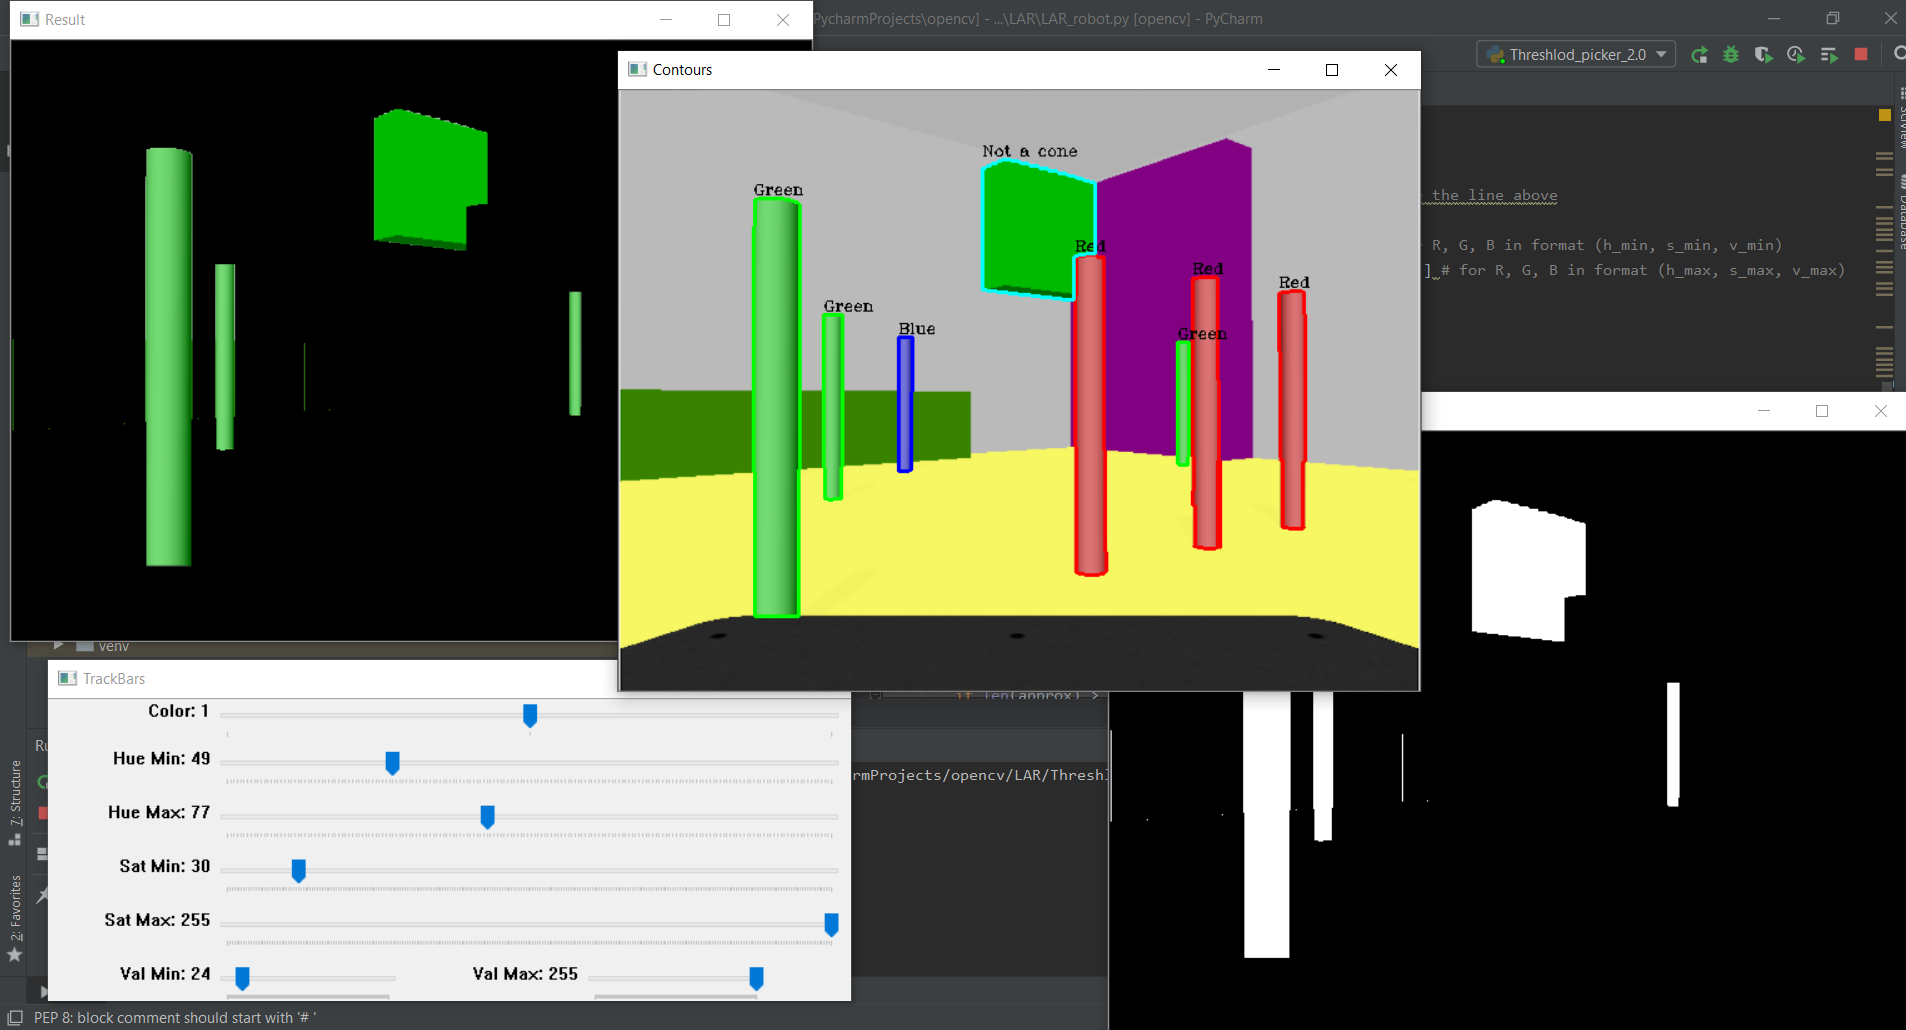
\includegraphics[width=\textwidth]{Threshold_Picker.png}
\caption{Pohled v aplikaci Threshold Picker 2.0}
\label{thr_picker}
\end{figure}
Dalším podpůrným skriptem je skript quaternion\_to\_rot\_matrix, který byl použit pouze jednou pro převedení quaternionu na rotační matici. Tento kód jsme převzali z \cite{quaterniony}.

\begin{thebibliography}{}

\bibitem{prezentace}
https://cw.fel.cvut.cz/wiki/\_media/courses/b3b33lar/petrik\_lar21\_en.pdf
\bibitem{quaterniony}
https://automaticaddison.com/how-to-convert-a-quaternion-to-a-rotation-matrix/
\end{thebibliography}
\end{document}


\end{document} 